\documentclass[12pt,twoside,a4paper]{article}
\usepackage{hyperref}
\usepackage{graphicx}
\usepackage[T1]{fontenc}
\usepackage[utf8]{inputenc}
\usepackage{enumitem}
\usepackage{array,tabularx}
\usepackage[a4paper,left=3cm,right=2cm,top=2.5cm,bottom=2.5cm]{geometry}
\usepackage{authblk}

\setlist[enumerate,1]{labelindent=0pt, leftmargin=*}
\pagestyle{empty}

\newcolumntype{P}{>{\centering\arraybackslash}p{0.75cm}}
\newcolumntype{L}{>{\raggedright\arraybackslash}m{0.2\textwidth}}
\newcolumntype{R}{>{\raggedleft\arraybackslash}m{0.2\textwidth}}

\newcommand{\usetbl}{%
  \begin{tabular}{@{}|*5{P|}@{}}
    \hline
    1 & 2 & 3 & 4 & 5 \\
    \hline
  \end{tabular}
}

\newcommand\prop[1]{%
  \item
  \parbox[t]{0.5\textwidth}{#1}%
  \qquad
  \parbox[t]{0.5\textwidth}{\usetbl}%
}

\graphicspath{{images/}}

\hypersetup{
    colorlinks=true,
    linkcolor=blue,
    filecolor=magenta,
    urlcolor=cyan,
    citecolor=black,
}

\title{BLAST: Hands-On Workshop}
\author[1]{Wehr, Thomas}
\author[2]{Fleiner, Christian}
\affil[1]{Supply-Chain-Services (SCS), Fraunhofer IIS}
\affil[2]{Chair of Technical Information Systems, FAU Erlangen-Nürnberg}
\date{June 15, 2021}

\renewcommand\Authands{ and }

\begin{document}

\maketitle

\section{Prerequisites}
Open BLAST (\href{https://paul.ti.rw.fau.de/~qa60fyri/campus/blast/}{https://paul.ti.rw.fau.de/~qa60fyri/campus/blast/}) in your favorite Browser.

\noindent BLAST is a visual programming environment used to create IoT-Applications by arranging blocks.

\begin{center}
  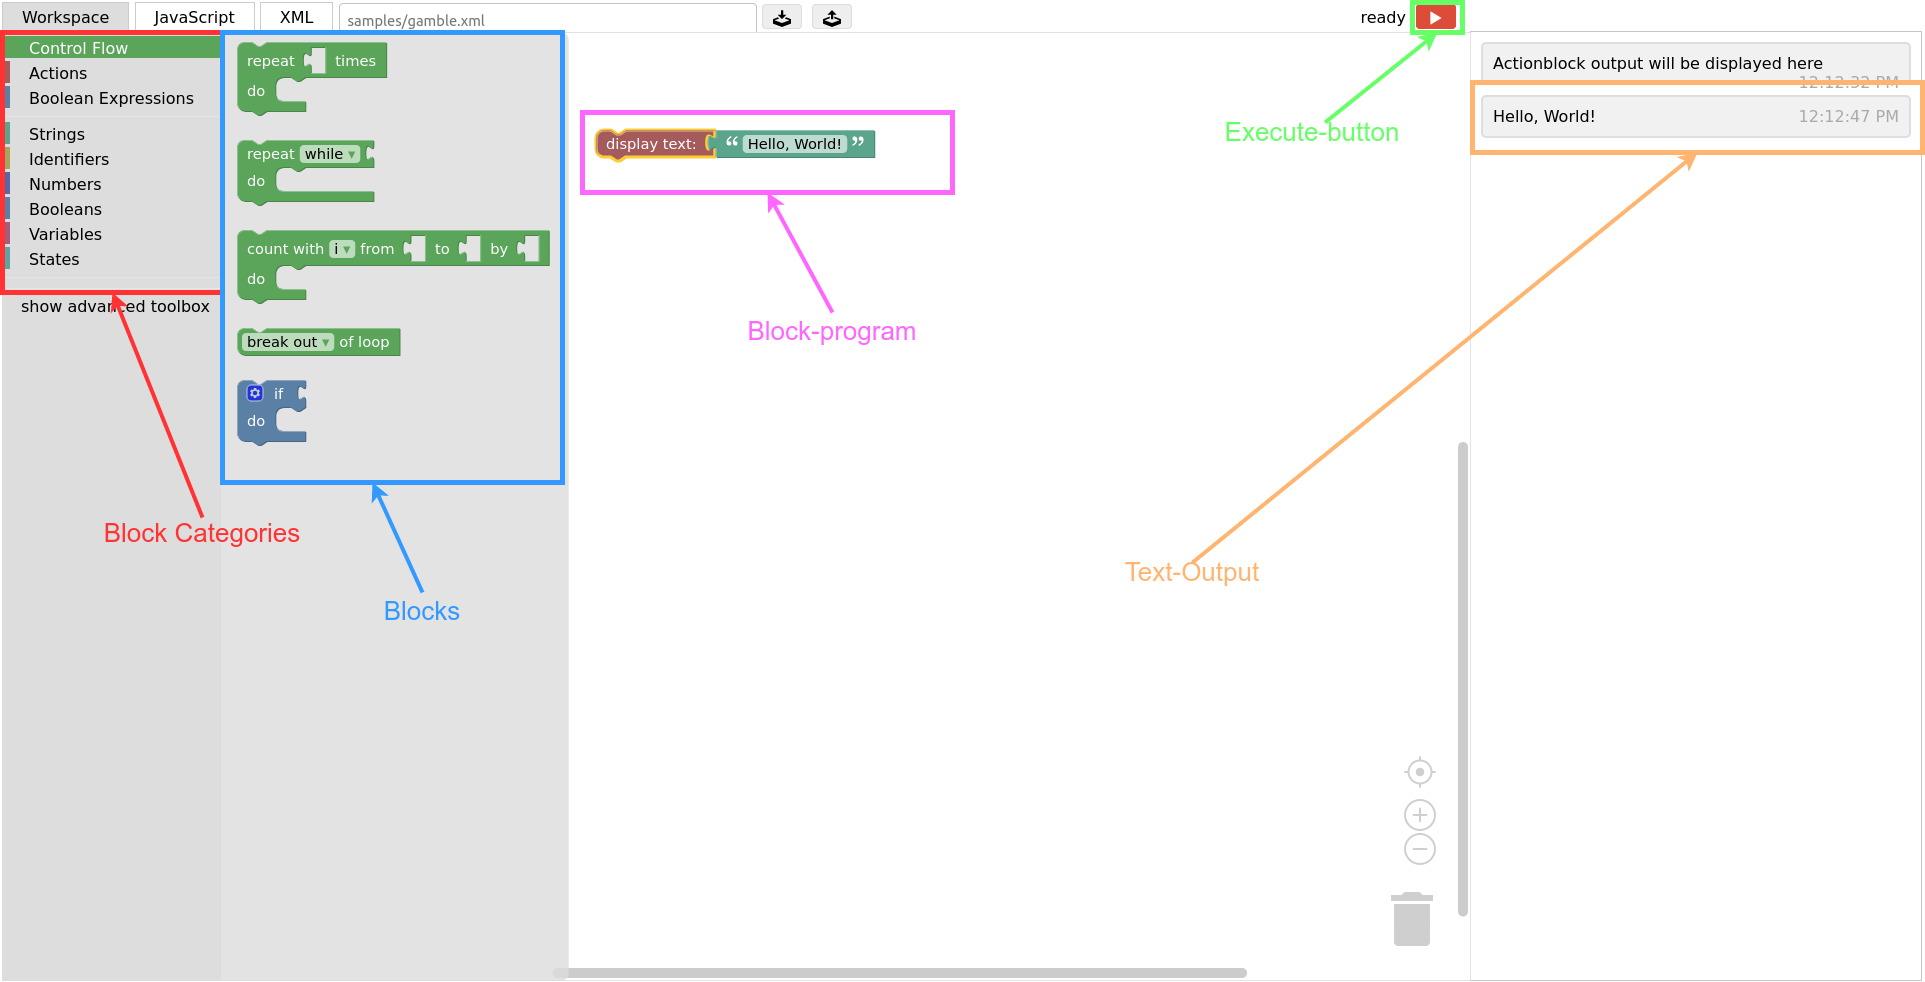
\includegraphics[width=\textwidth]{screenshot.png}
\end{center}

\section{Introductory exercises}
Solve the following exercises using the blocks provided by BLAST.
\subsection{Hello World!}
Create and execute a block-program displaying the message ``Hello, world!''.

Hint: You need the \textbf{display text} block to display messages and a \textbf{string} block to define a text.

\subsection{Variables}\label{sub:variables}
Create and execute a block-program, that successively displays the messages ``Hello, 1'', ``Hello, 2'' and ``Hello, 3''. Use a variable for the number.

Hint: Use arithmetic operations from the \textbf{Numbers} category to increment the variable.

\subsection{Loops}\label{sub:loops}
Extent the program of ~\ref{sub:variables}, but display messages for the numbers 1 to 10 and use only 1 \textbf{display text} block by adding a block from the \textbf{Control Flow} category.

\subsection{If clauses}
Skip each even number in the output of ~\ref{sub:loops} by using an \textbf{if} block.

Hint: The \href{https://en.wikipedia.org/wiki/Modulo_operation}{modulo operation}(\%) can be used to determine even numbers.

\end{document}